% !TeX spellcheck = en_GB
\chapter{Main Objectives}
\todo[inline]{we have to be careful with our terminology across different sections: what is the wiki? what is an article? anything in the wiki or just user created content?, what are 'information' in our case?, what is a 'problem'? what are 'users' outside of the user type section? what's a topic?}
\todo[inline]{each section if applicable should explain why? who? what? where? how?}

\section{Overview}
The goal of this project is to design, implement and provide a guidance platform for the developing country Afghanistan. 
Taking the circumstances in such a developing country in account, the platform should provide the users of IT-systems with the knowledge to assure the sustainability of IT-systems in their countries. 
Besides providing general information on IT-systems, the platform should provide, similar to the “BSI Grundschutzkatalog”, information aiming to localize and solve problems that may occur in the IT-systems as a result of a human error, technical failure or a catastrophe etc. 
\\
\begin{figure}[h] 
    \centering
    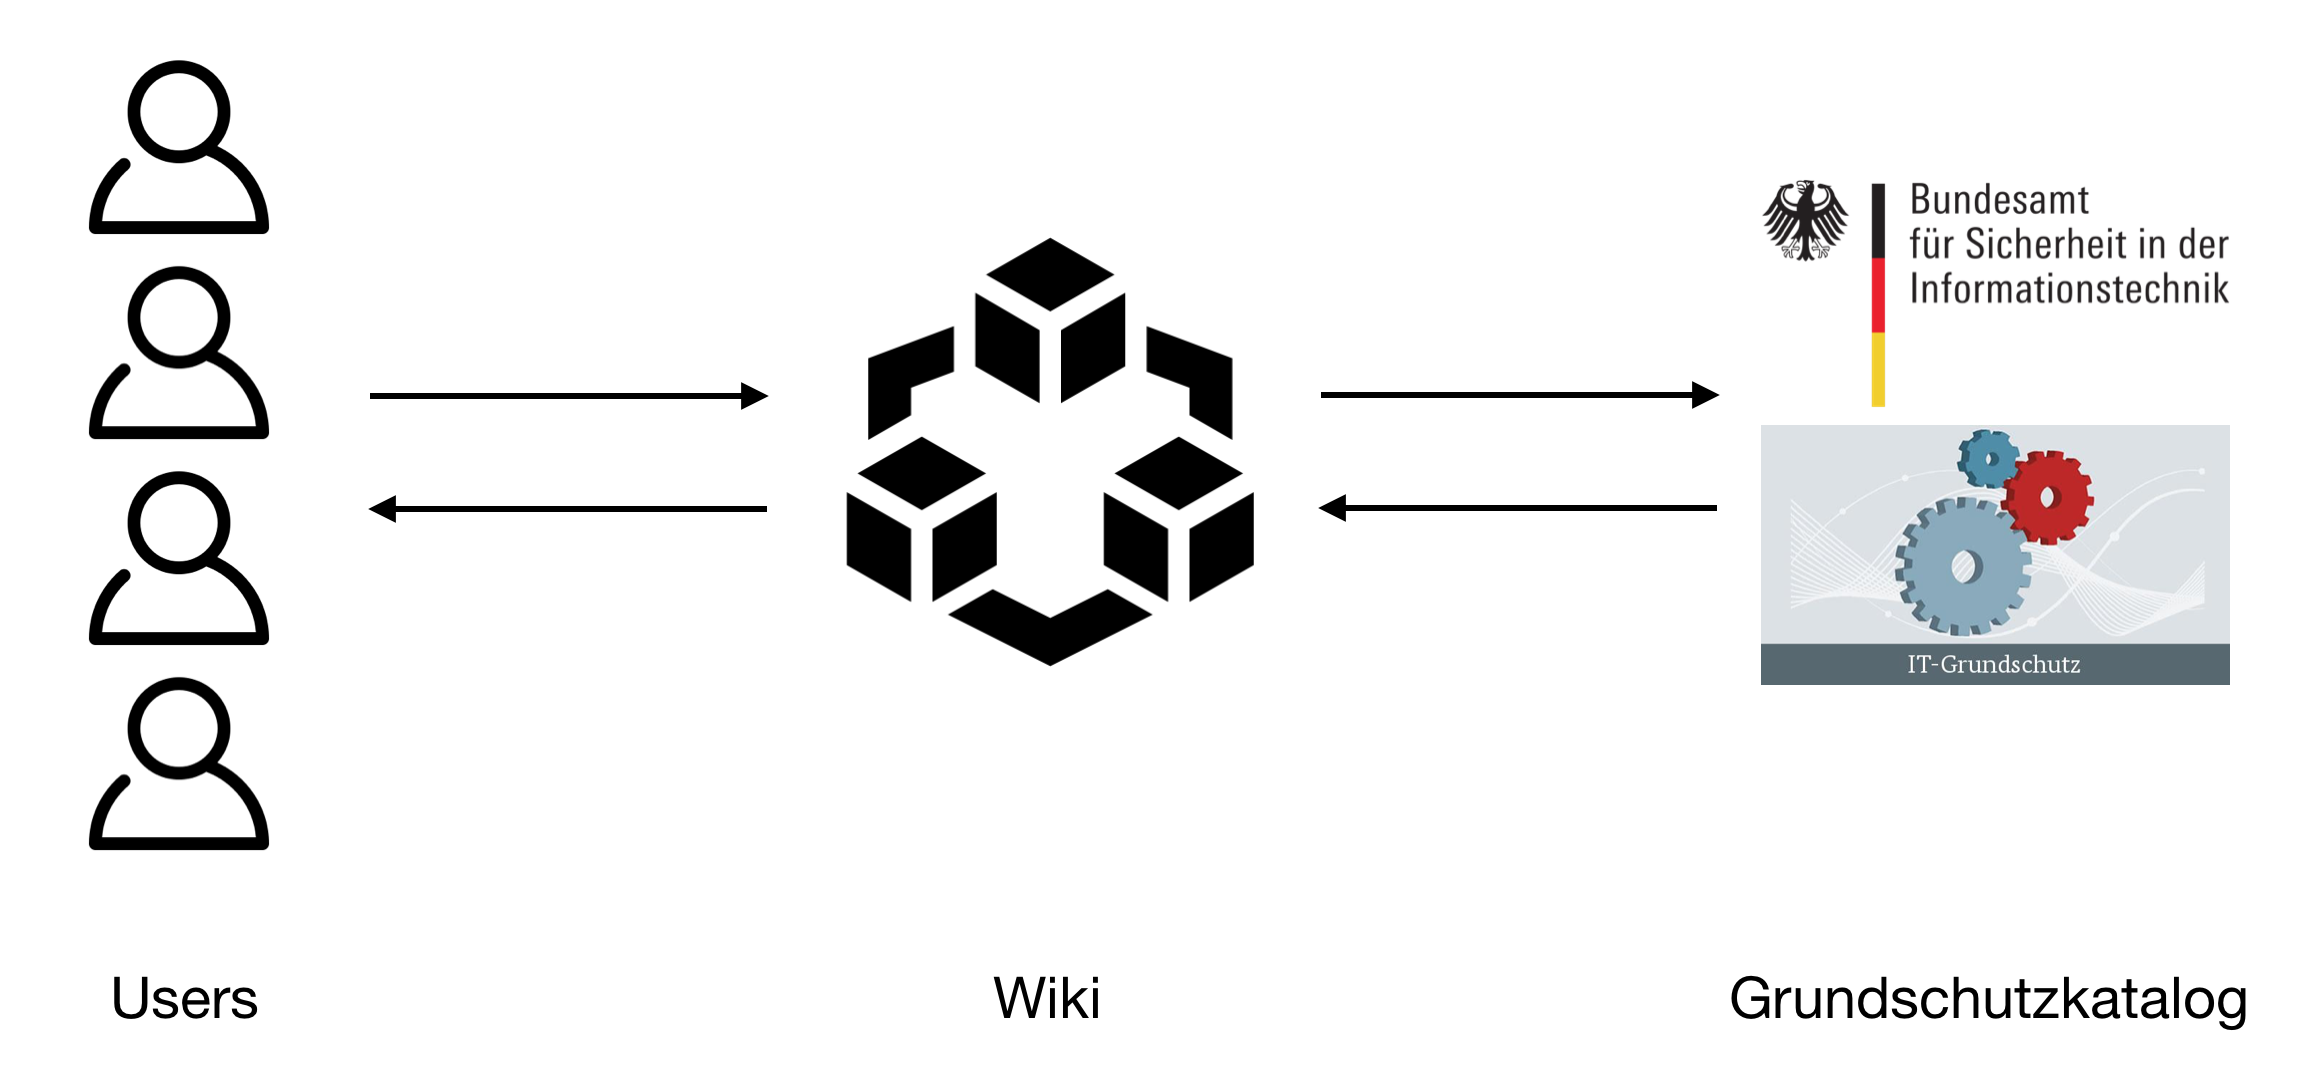
\includegraphics[scale=0.3]{Pictures/ConceptSketch}
    \caption{Abstract System Design}
\end{figure}


\section{Wiki} 
Considering the limited availability of IT-specialists in most of the developing countries, and after reviewing the possible ways to design and provide the platform, our team considers it convenient to create an open platform on which people can collaboratively add, edit, delete or archive content, similar to Wikipedia. 
This should allow the platform to constantly grow and stay relevant to current circumstances. 
However, this should not mean that everyone can write whatever content for everybody to read. 
To assure that we have to set rules and access permission levels (see section~\ref{user_types}). 
\todo[inline]{this explanation should be more detailed; how is the archive related to the wiki?, how is created content linked to the catalogue? in general, what is part of the wiki?}

\section{Archive}
\label{archive}
The website should always be up-to-date but we also want to offer the possibility to look up the old content.
For this we need an archive.
The archive stores information \todo[inline]{precisely what kind of information} that is no longer up-to-date but could still be relevant for some users. 
For example: if users are looking for a problem such as a no longer supported operating system and there are no information in the wiki regarding this problem, the user could find older approaches in the archive. 
\todo[inline]{what happens to content pages in the wiki which were linked to the catalogue? do they get archived?}

\section{User Types} 
\label{user_types}
First of all, the platform will need one or multiple administrators (admins) who will update the platform from a technical perspective and ensure that policies are being respected. 
However, building a wiki-like platform about IT-Security for developing countries comes also with big responsibility about the content it will provide. 
If everybody could publish and/or modify content without checks or labels for flaws, or malicious informations, would present a major security risk for any layman reading it. 
Admins will have enough workload so we need another team of volunteers, like moderators (mods), who will check content and remove, modify or label it as unsafe if necessary. 
Moderators will be appointed by admins and will be responsible for policy enforcement for specific topics. 
Further, users who would like to publish and/or modify content will need to register to the platform and be logged in. 
All other users who are not logged in will be considered as guests and will only be able to "read only" content. 
These multiple user roles are needed to create a trustworthy platform. 
\\\\
In the following section will be discussed the different user roles and their functions. 
%We decided to create four types of users with different user rights. 
This is illustrated in the appendix by the use case diagrams. 
\\
\textbf{Guest}, the guests have the possibility to browse and search in the archive and also in the wiki\todo[inline]{do we distinguish between wiki and catalogue or do we always also mean the catalogue when we just say wiki? compare to: the archive is just another part of the wiki}. 
The search can be refined with several options (more information about the search in the text search section~\ref{search_function}). 
If guests are not sure how to find their problems they can use the wizard (more information in the Wizard section~\ref{wizard}). 
The wiki contains news from different topics which guests can check out.

\textbf{User}, every registered\todo[inline]{how does a user register? important for how to effectively ban them} user can write articles in the wiki and change them with the functions: create content and edit content. 
They can also edit their profile. 
Users can use all functions guests can use.
\todo[inline]{they have to login}

\textbf{Moderator} (mod), mods will be appointed for a specific topic for example “b2 infrastructure”\todo[inline]{too brief; what exactly are topics and where are they/where relevant? catalogue, content, news, archive?, see BSI catalogue section where is written that only admins can edit the catalogue; appointed to a topic means they can still edit content from different topics?} . 
Mods are responsible for moderating articles, which means to delete wrong or inappropriate content or make it recognizable for users\todo[inline]{for user type users or website users?} that the article is unverified. 
They create the news\todo[inline]{didn't we say users can create news but only mods can put them on the homepage?}  and they are also responsible - if necessary - to ban users. 
Mods can use all functions users can use.

\textbf{Administrator} (admin), the admin is responsible for appointing the mods and remove them if necessary. 
He also manages the topics\todo[inline]{what, where} , which means creating new topics, removing old ones and controlling that each topic got a mod. 
For new topics or new mods, the admin sets new permissions \todo[inline]{what are the possible permissions}or changes them. 
One of the most important tasks of the admin is to update the BSI catalogue as soon as a new one is available and to move the old one to the archive. 
The admin can use all functions mods can use.
\todo[inline]{how many admins do we suggest, how many mods? redundancy}


\section{BSI Catalogue}
The English version of the BSI catalogue has been published in a single PDF file. 
This makes browsing, or even searching a specific problem, a difficult task for beginners. 
Therefore the BSI catalogue should be added as "locked" content to the wiki,\todo[inline]{whats an article -> changed word "article" to "content"? where? part of wiki; really only admins?} only modifiable by administrators.
\\\\
In fact, converting catalogues in articles by hand would be an extended task. 
Accordingly, a parser is needed. 
This parser will analyse the PDF file and create the article automatically. 
Further, the BSI provides cross-reference tables of the catalogue. 
These amend the useful links inside each subsection and could be used to recommend cross-referenced counter-measures to specific threats.\todo[inline]{how? -> i don't know yet}


\section{Text Search}
\label{search_function}
A text search function allows users of the platform to make a free text search request and browse the results containing the key-words. 
Users should also have the opportunity to narrow down their search request by selecting a specific domain \todo[inline]{maybe 'domain' would be better here?-DONE} in which they would like to find results:
\begin{itemize}
\item "All": counts as every domain
\item "News": domain where news are published
\item "Module": modules of the BSI Grundschutzkatalog
\item "Threats": threats of the BSI Grundschtzkatalog
\item "Measures": measures of the BSI Grundschutzkatalog
\item "Archive": archived content (no longer visible in the wiki)
\end{itemize}
\todo[inline]{briefly explain what those 'topics' mean-DONE } 
Choices should be available as a dropdown list.
\\\\
The search field should be well placed on the home page. 
The system should have a function "Back to the search results". 
The search function should have fault tolerance, as well as the ability to deal with synonyms. 
Fault tolerance means that the user will get the result even if he misspells a word or if he uses singular or plural. 
While a non-fault-tolerant search will let the visitor go nowhere, the system should nevertheless display the appropriate results.
In addition, search functions which also master synonyms, do even more. 
For example, the system should derive results from the search input "laptop" in which the word "notebook" appears and for this purpose access an extensive database of words of the same meaning. 
The automatic completion of search terms is very welcome.
 
\section{Wizard}
\label{wizard}
Beginners who are not familiar with the terminology may have a hard time finding solutions to problems they encounter. 
To help them, we would like to implement a wizard, which will ask them a set of yes/no questions to filter out what problems they could have, similar to the game Akinator\footnote{\url{http://en.akinator.com}}. 
 
\section{Home Page}
The home page is the entry point to the different services offered by the website. 
As such its design should provide a clear overview of and a dead on target guidance to all available functions for users of all levels of experience.
Firstly, the home page also displays the always present top section (see section~\ref{top_section}) but no side bar to use the full available space for the sections defined below and in order to not overwhelm the user with two detailed lists of items.
Directly below the top section is a distinguished area for time-critical news which inform of widespread threats or important updates.
Those are important to all users and should therefore be on top.
In times of no imminent danger time-critical news might not be displayed but instead a few of the most recent regular news which are part of the wiki.
The third area in a vertical sense is a wide and inviting search bar that allows experienced users the quick access to the BSI catalogue and other parts. 
Should a user not know what to search he can browse the BSI catalogue following a link in the top section (see section~\ref{top_section}).
The search offers the full functionality as described in section~\ref{search_function}.
As a last section before the always present bottom section is an overview of introductory tutorials on how to implement the guidelines of the BSI catalogue while developing, building and maintaining a basic IT system.
Equally visible as the tutorials should be the offer to use the wizard to help and find security gaps and other system flaws.
Both the tutorials and the wizard are aimed at users of no or little knowledge or overview of the BSI catalogue.
For detailed explanations see section~\ref{tutorials} for the tutorials and section~\ref{wizard} for the wizard.
The bottom section shows links to items as contact, legal notice, possibly FAQ and copyright.

\begin{figure}[h]
    \centering
    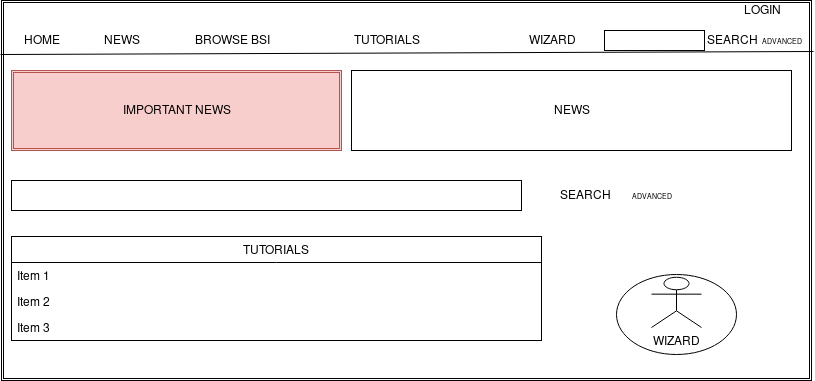
\includegraphics[scale=0.3]{Pictures/frontpage_mockup}
    \caption{Schematic Frontpage Design}
\end{figure}
 
\section{Top Section} 
\label{top_section}

The top section is an always present area at the top of each subpage that connects the different services and allows for quick access.
It should feature the following items whose order and wording might be changed appropriately:
\begin{itemize}
    \item Home/Frontpage
    \item News
    \item Browse the BSI catalogue
    \item Tutorials
    \item Wizard
    \item Search
    \item Login 
        . 
\end{itemize}


%\section{Tutorials}
%\label{tutorials}

%Tutorials should call unexperienced users' attention to the most important points in the BSI catalogue when developing, building or maintaining an IT infrastructure.
%They could briefly explain mayor points of the BSI catalogue and indicate next steps.
%The simplest tutorial could simply introduce the usage and goal of the website and its subservices.
%The tutorials are not meant to be a rewrite - i.e. the BSI catalogue for dummies - but thought of as a quick overview and guiding introduction into the matter.
%They are part of the wiki and as such created and maintained by content manager and linked by mods.
%\todo[inline]{to remove?}
